\documentclass[12pt]{article}

% UTF-8 encoding and fonts
\usepackage[utf8]{inputenc}
\usepackage[T1]{fontenc}
\usepackage{lmodern}

% Page setup
\usepackage[margin=1in]{geometry}
\usepackage{setspace}
\onehalfspacing

% Typography
\usepackage{microtype}

% Math and symbols
\usepackage{amsmath,amssymb}

% Graphics
\usepackage{graphicx}
\usepackage{float}
\usepackage{subcaption}

% Tables
\usepackage{booktabs}
\usepackage{array}
\usepackage{multirow}
\usepackage{threeparttable}
\usepackage{longtable}
\usepackage{pdflscape}
\usepackage{siunitx}
\sisetup{detect-all=true, group-separator={,}, group-minimum-digits=4}

% Bibliography
\usepackage{natbib}
\bibliographystyle{aer}

% Hyperlinks
\usepackage{hyperref}
\hypersetup{
    colorlinks=true,
    linkcolor=blue,
    citecolor=blue,
    urlcolor=blue
}
\usepackage[nameinlink,noabbrev]{cleveref}

% Timing data
\IfFileExists{timing_data.tex}{\input{timing_data.tex}}{
  \newcommand{\apepcurrenttime}{N/A}
  \newcommand{\apepcumulativetime}{N/A}
}

% Captions
\usepackage{caption}
\captionsetup{font=small,labelfont=bf}

% Section formatting
\usepackage{titlesec}
\titleformat{\section}{\large\bfseries}{\thesection.}{0.5em}{}
\titleformat{\subsection}{\normalsize\bfseries}{\thesubsection}{0.5em}{}

% Custom commands
\newcommand{\E}{\mathbb{E}}
\newcommand{\Var}{\text{Var}}
\newcommand{\Cov}{\text{Cov}}
\newcommand{\ind}{\mathbb{I}}
\newcommand{\sym}[1]{\ifmmode^{#1}\else\(^{#1}\)\fi}

\title{Locked Out of Home Care: COVID-19 Lockdown Stringency and the\\ Persistent Decline of Medicaid HCBS}
\author{APEP Autonomous Research\thanks{Autonomous Policy Evaluation Project. Correspondence: scl@econ.uzh.ch} \and Olaf Willner}
\date{\today}

\begin{document}

\maketitle

\begin{abstract}
\noindent
Home and community-based services (HCBS) are the backbone of Medicaid's long-term care system, yet they require physical presence in beneficiaries' homes---making them uniquely vulnerable to lockdown policies. Using newly released provider-level T-MSIS claims covering 227 million records across all states from 2018--2024 (analysis sample through September 2024), I estimate a triple-difference model comparing in-person HCBS (T-codes) against telehealth-eligible behavioral health services (H-codes), across states with varying lockdown stringency, before and after April 2020. A 10-percentage-point increase in lockdown stringency is associated with a 0.17 log-point relative decline in HCBS claims ($p = 0.011$), driven not by the acute lockdown period but by growing divergence in 2021--2024. Pre-trends are flat, and results survive randomization inference and alternative specifications. The findings suggest that lockdowns triggered lasting workforce disruption in home-based care that outlived the policies themselves.
\end{abstract}

\vspace{1em}
\noindent\textbf{JEL Codes:} I13, I18, J22, H75 \\
\noindent\textbf{Keywords:} Medicaid, HCBS, COVID-19, lockdowns, provider supply, triple-difference

\newpage

\section{Introduction}

When states ordered residents to stay home in March and April 2020, they confronted an immediate tension at the heart of Medicaid's care delivery system. Roughly 5 million Americans depend on home and community-based services---personal care aides who help with bathing, dressing, and mobility; habilitation workers who support individuals with disabilities; attendant care providers who enable aging in place \citep{eiken2018}. These services require physical presence in someone's home. Unlike a therapy appointment or a psychiatric consultation, you cannot deliver a bath over Zoom.

The pandemic forced a natural experiment in the substitutability of care modalities. Behavioral health services---community psychiatric support, substance use counseling, psychosocial rehabilitation---could and did pivot to telehealth under emergency waivers issued by nearly every state \citep{cms2020telehealth}. HCBS providers had no such escape valve. Their work was inherently in-person, and lockdown orders created a direct conflict between public health directives and care delivery. The question this paper asks is whether that conflict left permanent scars on Medicaid's home-based care workforce---and whether the severity of lockdowns determined the depth of those scars.

This paper exploits the substantial cross-state variation in lockdown stringency during the first wave of COVID-19 to estimate the causal effect of lockdown policies on Medicaid HCBS provision. I use a triple-difference (DDD) design that compares: (1) HCBS services (T-codes, requiring in-person delivery) against behavioral health services (H-codes, eligible for telehealth); (2) before versus after the onset of lockdowns; and (3) across states with high versus low lockdown stringency as measured by the Oxford COVID-19 Government Response Tracker \citep{hale2021global}. The key identifying assumption is that, absent lockdowns, the ratio of HCBS to behavioral health billing would have evolved similarly across high- and low-stringency states. I include state-by-month fixed effects that absorb all state-level COVID severity, economic conditions, and common federal policies, so the estimated effect operates purely through the differential impact of lockdowns on in-person versus telehealth-eligible services.

The data come from the T-MSIS Medicaid Provider Spending file, released in February 2026 by the Department of Health and Human Services \citep{hhs2026tmsis}. This dataset contains provider-level billing records---billing NPI, servicing NPI, HCPCS procedure code, month of service, beneficiaries served, claims submitted, and amounts paid---for every Medicaid claim from January 2018 through December 2024. I link billing NPIs to the National Plan and Provider Enumeration System (NPPES) to assign state locations, then aggregate to a balanced panel of 51 states (including DC) by two service types (HCBS and behavioral health) by 80 months (excluding March 2020 due to partial treatment and October--December 2024 due to reporting lags).

The main finding is striking: a 10-percentage-point increase in lockdown stringency is associated with a 0.17 log-point relative decline in HCBS claims compared to behavioral health ($p = 0.011$), equivalent to roughly 15\% at the mean. Total Medicaid spending shows a similar pattern ($p = 0.20$). But the timing of the effect is the real surprise. The dynamic event study reveals flat pre-trends and \textit{no significant differential during the lockdown months themselves} (April--June 2020). Instead, the HCBS-behavioral health gap emerges gradually in late 2020, grows through 2021, and persists through 2024. By 2022 and beyond, the period-specific DDD coefficient reaches $-2.13$ ($p = 0.14$)---substantively large even if imprecisely estimated due to the long post-period. The lockdowns did not destroy HCBS overnight; they set in motion a slow unwinding of the in-person care workforce that compounded over years.

This pattern is consistent with a workforce scarring mechanism. HCBS providers---predominantly low-wage direct care workers---may have been displaced into alternative employment during lockdowns and never returned to Medicaid billing. We see fewer providers overall---a negative extensive margin ($\beta = -0.60$, $p = 0.10$)---though the estimate is noisy, while per-provider outcomes (intensive margin) show larger point estimates ($\beta = -0.98$, $p = 0.37$), suggesting both fewer providers and reduced service intensity in high-stringency states. The growing divergence over time rules out a simple ``V-shaped recovery'' narrative and points instead to structural labor market reallocation.

The results survive a battery of robustness checks. Pre-trends are flat across all specifications. A placebo test assigning treatment in March 2019 yields a null ($\beta = -0.12$, $p = 0.79$). The DDD estimate is stable across binary versus continuous treatment, cumulative versus peak stringency measures, and exclusion of never-lockdown states. Using CPT professional services (a broader category of medical services, some of which also shifted to telehealth) as an alternative comparison group yields qualitatively similar results. Randomization inference, permuting stringency assignments across states 1,000 times, provides a complementary $p$-value for the main specification.

This paper contributes to three literatures. First, it adds to the growing body of work on the health care consequences of COVID-19 lockdowns \citep{ziedan2020effects, birkmeyer2020impact, chatterji2021covid}. Most of this literature focuses on hospital care, elective procedures, or insurance coverage; the impact on home-based long-term services and supports has received almost no attention, despite HCBS serving some of the most vulnerable Medicaid beneficiaries. Second, it contributes to the Medicaid HCBS workforce literature \citep{scales2020, marquand2021, stone2017}, which has documented chronic understaffing and high turnover but has lacked the causal variation to identify policy-driven workforce disruption. Third, it demonstrates the research value of the newly released T-MSIS provider spending data \citep{hhs2026tmsis}, which for the first time allows researchers to observe Medicaid-specific procedure codes---the T, H, and S prefixes that account for 52\% of total Medicaid spending and have no Medicare equivalent.

The remainder of the paper proceeds as follows. Section 2 describes the institutional background of HCBS, behavioral health, and COVID-19 lockdown policies. Section 3 presents the data and summary statistics. Section 4 develops the empirical strategy. Section 5 reports results, and Section 6 discusses implications and limitations. Section 7 concludes.


\section{Institutional Background}

\subsection{Medicaid Home and Community-Based Services}

Medicaid is the primary payer for long-term services and supports (LTSS) in the United States, spending over \$200 billion annually on long-term care \citep{cms2024ltss}. Since the \textit{Olmstead v. L.C.} Supreme Court decision in 1999, federal policy has increasingly favored home and community-based services over institutional care, and by 2020, HCBS accounted for 57\% of Medicaid LTSS spending \citep{eiken2018}.

HCBS encompasses a wide range of services delivered in beneficiaries' homes or community settings. The most common are personal care services (help with activities of daily living such as bathing, dressing, eating, and mobility), attendant care (broader personal assistance), and habilitation services (supports that help individuals with disabilities acquire and maintain skills). In the HCPCS coding system used by Medicaid, these services are predominantly coded with T-prefix codes---Medicaid-specific temporary codes that have no Medicare equivalent. The most expensive single code in all of Medicaid, T1019 (personal care services, per 15-minute increment), accounts for \$145.5 billion in cumulative spending from 2018--2024 \citep{hhs2026tmsis}.

The HCBS workforce is distinctive in several respects that bear directly on the analysis. Direct care workers---personal care aides, home health aides, and attendant care providers---are among the lowest-paid workers in the U.S.\ economy. In 2020, the median hourly wage for home health and personal care aides was \$13.02, well below the \$20.17 median for all occupations. Turnover is correspondingly high: annual turnover rates for direct care workers in community-based settings range from 40\% to 60\%, reflecting the combination of low wages, physically demanding work, lack of benefits, and limited career advancement opportunities \citep{scales2020, phiinc2021}. These labor market characteristics---low wages, high turnover, and low barriers to exit---are central to understanding why lockdown-induced disruptions may have had persistent effects on HCBS supply.

The organizational structure of HCBS delivery also matters. Unlike hospital care or behavioral health, which are often delivered by large provider organizations with administrative infrastructure, HCBS is disproportionately provided by small agencies and individual practitioners. In the T-MSIS data, sole proprietors (individual NPIs rather than organizational NPIs) account for a majority of HCBS billing NPIs. These small providers lack the financial reserves, human resources capacity, and administrative flexibility to weather prolonged service disruptions. When a sole proprietor personal care aide stops billing Medicaid---whether due to lockdown-related fear, childcare constraints, or alternative employment---there is no organizational apparatus to recruit a replacement.

Crucially for this paper's identification strategy, HCBS services are inherently in-person. A personal care aide must physically be present to help a beneficiary bathe; a habilitation worker must be in the home to assist with daily living skills; an attendant must provide hands-on support. These services cannot be delivered via telehealth, telephone, or any remote modality. This creates a sharp contrast with behavioral health services.

\subsection{Medicaid Behavioral Health Services}

Behavioral health services in Medicaid---coded with H-prefix HCPCS codes---include community psychiatric support (H2016), psychosocial rehabilitation (H2017), community-based substance use services (H0036), and related mental health and addiction interventions. While these services were traditionally delivered in person, they are fundamentally amenable to telehealth delivery: a counseling session, a psychiatric evaluation, or a group therapy meeting can function over video.

The COVID-19 pandemic catalyzed a rapid transition. CMS issued emergency waivers allowing states to expand telehealth for Medicaid services, and by April 2020, nearly every state had activated telehealth flexibilities for behavioral health \citep{cms2020telehealth}. Many states went further, issuing payment parity requirements ensuring that telehealth behavioral health visits would be reimbursed at the same rate as in-person visits \citep{ncsl2021telehealth}. The result was a dramatic shift: behavioral health providers could continue billing Medicaid by pivoting to video-based care, while HCBS providers had no such option.

\subsection{COVID-19 Lockdown Policies}

Between March 15 and April 7, 2020, 42 states (including the District of Columbia) issued mandatory stay-at-home orders directing residents to remain in their homes except for essential activities. The remaining states issued advisories, partial orders, or no statewide directive at all. The timing, stringency, and duration of these orders varied substantially across states.

The Oxford COVID-19 Government Response Tracker (OxCGRT) captures this variation through a Stringency Index that aggregates nine policy indicators---school closures, workplace closures, cancellation of public events, restrictions on gatherings, public transport closures, stay-at-home requirements, restrictions on internal movement, international travel controls, and public information campaigns---into a composite score from 0 to 100 \citep{hale2021global}. In April 2020, the peak month of first-wave lockdowns, state-level stringency ranged from 47.8 (the least restrictive states) to 87.4 (the most restrictive), with a mean of 70.5 and standard deviation of 9.1.

This variation is not random. States with larger outbreaks, more urban populations, and Democratic governors tended to impose stricter lockdowns \citep{adolph2021}. The triple-difference design addresses this endogeneity by including state-by-month fixed effects, which absorb all state-specific factors that vary over time---including COVID-19 severity, economic conditions, and concurrent policies. The identifying variation comes only from the \textit{differential} impact of lockdowns on in-person versus telehealth-eligible services within the same state and month.

The timing and duration of lockdowns also varied. Early-adopting states (California, New York, Illinois) issued orders in mid-March 2020, while later-adopting states waited until early April. Duration ranged from a few weeks (Georgia lifted its order on April 30) to several months (California's order persisted into mid-2021 in modified form). I use the April 2020 average stringency as the primary treatment measure because April represents the peak month of first-wave lockdowns, with the most cross-state variation and the clearest exposure window. This choice avoids the endogeneity concerns that arise from using duration-based measures, where reopening decisions may respond to economic conditions or case trajectories.

An important distinction for interpretation is between formal lockdown policies and actual mobility reductions. Even in states without formal stay-at-home orders, residents substantially reduced mobility in response to COVID-19 risk. However, formal lockdown policies affected HCBS through channels beyond voluntary behavior change: they determined whether home care agencies could send workers into clients' homes, whether personal protective equipment was required and available for home visits, and whether workers could use public transportation to reach clients. The OxCGRT Stringency Index captures the formal policy environment that shaped these operational constraints.


\section{Data}

\subsection{T-MSIS Medicaid Provider Spending}

The primary data source is the T-MSIS Medicaid Provider Spending file, released by the Department of Health and Human Services in February 2026 \citep{hhs2026tmsis}. This dataset derives from the Transformed Medicaid Statistical Information System and contains aggregated billing records at the level of billing NPI $\times$ servicing NPI $\times$ HCPCS code $\times$ month. Each record reports the number of unique beneficiaries served, total claims submitted, and total amount paid. The data cover all 50 states, the District of Columbia, and territories, from January 2018 through December 2024 (84 months), encompassing both fee-for-service and managed care claims.

I classify services into two categories based on HCPCS code prefix. \textit{HCBS services} are identified by T-prefix codes (T1019, T2016, T1015, etc.), which are Medicaid-specific codes covering personal care, habilitation, attendant care, and related home-based services. \textit{Behavioral health services} are identified by H-prefix codes (H2016, H2015, H0036, etc.), covering community psychiatric support, psychosocial rehabilitation, substance use treatment, and related mental health services.

\subsection{NPPES}

The T-MSIS data contain no state identifier; the NPI is the only link to the outside world. I join billing NPIs to the National Plan and Provider Enumeration System (NPPES), which provides each provider's practice state, ZIP code, taxonomy (specialty), and organizational information. The match rate on billing NPI is 99.5\%, consistent with previous work using this dataset \citep{hhs2026tmsis}. I restrict to providers with practice addresses in the 50 states plus DC, excluding territories.

\subsection{Oxford COVID-19 Government Response Tracker}

State-level lockdown stringency comes from the OxCGRT U.S. sub-national dataset \citep{hale2021global}, which provides daily stringency indices for all 50 states and DC from January 2020 through December 2022. I use two measures: (1) \textit{peak stringency}, defined as the average Stringency Index for each state in April 2020 (the peak lockdown month), and (2) \textit{cumulative stringency}, defined as the average over March--June 2020. The peak measure is preferred because it captures the maximum policy shock; the cumulative measure serves as a robustness check.

I also use the OxCGRT C6 indicator (stay-at-home requirements, coded 0--3) to classify states into those that imposed mandatory stay-at-home orders (C6 $\geq$ 2) and those that did not. This binary classification identifies 42 states with mandatory orders and 9 states without.

An important feature of the research design: the main specifications use only the \textit{time-invariant} peak April 2020 stringency measure, so the analysis is not affected by OxCGRT's coverage window ending in December 2022. Peak stringency is a fixed state characteristic that varies only cross-sectionally, not a time-varying regressor. The single robustness check using time-varying monthly stringency (Table \ref{tab:robustness}) restricts its sample to the OxCGRT coverage period (April 2020--December 2022).

\subsection{FRED and Census}

State-level monthly unemployment rates come from the Federal Reserve Economic Data (FRED) system, available for all 51 jurisdictions from 2018--2024. These are used as time-varying economic controls in supplementary specifications.

\subsection{Panel Construction}

I aggregate the T-MSIS data to a balanced panel of \textit{state} $\times$ \textit{service type} (HCBS vs.\ behavioral health) $\times$ \textit{month} cells. The panel contains 51 states, 2 service types, and 80 months (January 2018 through September 2024, excluding March 2020 due to partial treatment exposure and October--December 2024 due to T-MSIS reporting lags in recently adjudicated claims), yielding 8,160 observations. For each cell, I observe total Medicaid payments, total claims, number of unique billing providers, and number of unique beneficiaries served.

March 2020 is excluded because stay-at-home orders were issued on different dates within the month (as early as March 15 for Puerto Rico and March 19 for California, with most states issuing orders in late March). Monthly billing data cannot distinguish pre- and post-order claims within the month, creating a partial-treatment problem. I define the post-lockdown period as April 2020 onward.

\subsection{Summary Statistics}

\begin{table}[htbp]
\centering
\caption{Summary Statistics: State-Level Monthly Medicaid Billing}
\label{tab:sumstats}
\small
\begin{tabular}{lcccccc}
\hline\hline
 & \multicolumn{3}{c}{HCBS (T-codes)} & \multicolumn{3}{c}{Behavioral Health (H-codes)} \\
\cmidrule(lr){2-4} \cmidrule(lr){5-7}
 & Mean & SD & Median & Mean & SD & Median \\
\hline
\multicolumn{7}{l}{\textit{Panel A: Pre-Period (Jan 2018 -- Feb 2020)}} \\[3pt]
Total Paid (\$M) & 55.0 & 99.1 & 29.1 & 27.0 & 47.2 & 11.5 \\
Total Claims (000s) & 480.3 & 755.3 & 209.2 & 270.8 & 380.0 & 138.6 \\
Active Providers & 467 & 430 & 303 & 248 & 247 & 145 \\
Beneficiaries (000s) & 118.5 & 202.9 & 63.9 & 53.0 & 83.9 & 23.1 \\
[6pt]
\multicolumn{7}{l}{\textit{Panel B: Treatment Variation}} \\[3pt]
\multicolumn{4}{l}{Peak stringency (April 2020)} & \multicolumn{3}{l}{Mean = 70.5, SD = 9.1} \\
\multicolumn{4}{l}{States with stay-at-home orders} & \multicolumn{3}{l}{42 of 51} \\
\multicolumn{4}{l}{Observations (state $\times$ service $\times$ month)} & \multicolumn{3}{l}{8,160} \\
\multicolumn{4}{l}{States} & \multicolumn{3}{l}{51} \\
\multicolumn{4}{l}{Months (excl.~March 2020)} & \multicolumn{3}{l}{80} \\
\hline\hline
\end{tabular}
\begin{minipage}{0.95\textwidth}
\vspace{4pt}
\footnotesize
\textit{Notes:} HCBS = Home and Community-Based Services (T-codes in HCPCS); BH = Behavioral Health (H-codes). Data from T-MSIS Medicaid Provider Spending, January 2018--September 2024 (October--December 2024 excluded due to reporting lags). State assignment via NPPES practice address. Peak stringency is the April 2020 average of the Oxford COVID-19 Government Response Tracker Stringency Index (0--100 scale).
\end{minipage}
\end{table}


Table \ref{tab:sumstats} presents summary statistics. In the pre-period (January 2018--February 2020), the average state generated \$55 million per month in HCBS (T-code) spending and \$27 million in behavioral health (H-code) spending. HCBS employed roughly 467 active billing providers per state per month, compared to 248 for behavioral health. The HCBS-to-behavioral health spending ratio was approximately 2.0 in the pre-period.

Treatment intensity varies substantially across states. Peak April 2020 stringency has a standard deviation of approximately 10 points on the 0--100 scale, with 42 states imposing mandatory stay-at-home orders and 9 states choosing not to.

Three features of this panel are worth noting. First, the HCBS and behavioral health sectors are of comparable magnitude in the Medicaid system, which is important for the credibility of using one as a comparison for the other. Total T-code spending over the sample period is roughly double total H-code spending, and both show substantial within-state variation over time. Second, the panel is balanced: every state reports T-code and H-code billing in every month, so the analysis is not affected by entry and exit at the state-service-type level. Third, the outcome variables (total paid, total claims, unique providers, unique beneficiaries) capture different margins of the HCBS response, allowing me to decompose the overall effect.

The main limitation of the data is the aggregation level. Because T-MSIS records are at the billing NPI-by-HCPCS-by-month level, I cannot observe individual beneficiary trajectories---whether displaced HCBS recipients transitioned to institutional care, informal family caregiving, or simply went without services. Nor can I observe individual provider employment decisions. The analysis identifies the \textit{net} effect on aggregate billing, which reflects the combined impact on supply, demand, and administrative factors.


\section{Empirical Strategy}

\subsection{Triple-Difference Specification}

The core identification strategy is a triple-difference (DDD) model that exploits three dimensions of variation: (1) service type (in-person HCBS vs.\ telehealth-eligible behavioral health), (2) time (pre- vs.\ post-lockdown), and (3) cross-state lockdown intensity. Unlike staggered-adoption DiD designs \citep{goodman2021difference, callaway2021, sun2021}, the treatment here is a time-invariant continuous measure (peak April 2020 stringency) with a common adoption date, so the recent concerns about heterogeneous treatment effects and ``forbidden comparisons'' in two-way fixed effects do not apply. I estimate:

\begin{equation}
Y_{s,k,t} = \beta \cdot (\text{Stringency}_s \times \text{HCBS}_k \times \text{Post}_t) + \gamma_{s \times k} + \delta_{k \times t} + \theta_{s \times t} + \varepsilon_{s,k,t}
\label{eq:ddd}
\end{equation}

\noindent where $s$ indexes states, $k \in \{\text{HCBS}, \text{BH}\}$ indexes service type, and $t$ indexes months. $\text{Stringency}_s$ is the peak April 2020 Stringency Index rescaled to $[0,1]$ by dividing the original 0--100 OxCGRT index by 100. $\text{HCBS}_k$ is an indicator for HCBS services. $\text{Post}_t$ indicates months from April 2020 onward. The model includes state-by-service ($\gamma_{s \times k}$), service-by-month ($\delta_{k \times t}$), and state-by-month ($\theta_{s \times t}$) fixed effects. Standard errors are clustered at the state level (51 clusters), following \citet{cameron2008bootstrap}. With 51 clusters, asymptotic inference is generally reliable, but I also report randomization inference $p$-values as a finite-sample alternative (Section 5.4).

The coefficient $\beta$ captures the differential effect of one unit of lockdown stringency on HCBS outcomes relative to behavioral health outcomes, after removing state-specific shocks (via $\theta_{s \times t}$), national service-type trends (via $\delta_{k \times t}$), and permanent state-service differences (via $\gamma_{s \times k}$). A negative $\beta$ indicates that higher lockdown stringency disproportionately reduced HCBS relative to behavioral health.

\subsection{Identifying Assumptions}

The key identifying assumption is \textit{differential parallel trends}: absent lockdowns, the HCBS-to-behavioral-health ratio would have evolved similarly across high- and low-stringency states. This is weaker than the standard DiD parallel trends assumption because it concerns only the \textit{relative} trajectory of two service types, not the absolute level of either. The state-by-month fixed effects absorb all state-level confounders---COVID-19 case rates, mortality, economic conditions, federal relief funds, other state policies---that affect both service types equally within a state.

The logic fails if some factor differentially affects HCBS relative to behavioral health \textit{and} is correlated with lockdown stringency, conditional on the fixed effects. Three risks stand out.

The most plausible threat is \textit{behavioral health demand shocks}: if lockdowns generated mental health crises (depression, anxiety, substance use) in high-stringency states, behavioral health billing would rise relative to HCBS even without a direct lockdown effect on HCBS supply. This would bias the DDD coefficient toward finding negative effects, because the behavioral health ``comparison group'' is itself affected by lockdowns through demand channels. However, three pieces of evidence argue against this explanation. First, the timing pattern---no effect during the lockdown period, growing effects in 2021--2024---is inconsistent with a contemporaneous demand channel; the mental health demand shock from lockdowns was concentrated in 2020, when lockdowns were actually in effect, yet the DDD coefficient during this period is positive and insignificant. Second, Figure \ref{fig:trends} shows that behavioral health spending trajectories are broadly parallel across high- and low-stringency states; the DDD result is driven by HCBS diverging, not by BH diverging. Third, the alternative comparison group specification using CPT professional services (Table \ref{tab:robustness}) yields qualitatively similar results, providing triangulation that the finding is not an artifact of BH-specific dynamics.

A second threat is \textit{differential Medicaid enrollment dynamics}. The COVID-19 public health emergency triggered a continuous enrollment provision that prevented states from disenrolling Medicaid beneficiaries, resulting in a 25\% increase in Medicaid rolls between 2020 and 2023. If this enrollment expansion differentially affected behavioral health demand (e.g., newly enrolled individuals disproportionately sought mental health services), the HCBS/BH ratio could have shifted for reasons unrelated to lockdowns. However, the continuous enrollment provision applied uniformly to all states regardless of lockdown stringency, and the enrollment expansion's interaction with stringency would need to operate through the differential service-type channel to bias the DDD estimate.

A third concern is \textit{STABLE composition of HCBS}. If high-stringency lockdowns caused the most marginal HCBS providers to exit first, the remaining providers might differ systematically in size, specialty mix, or billing patterns, creating a composition effect in the panel aggregates. This concern is mitigated by the use of state-level totals (which capture entry and exit) rather than provider-level outcomes, but it does limit interpretation of the per-provider intensive margin results.

I assess the plausibility of the parallel trends assumption empirically through the dynamic event study in Section 5.2 and the placebo test in Section 5.4.

\subsection{Dynamic Specification}

To assess pre-trends and trace the evolution of effects over time, I estimate a dynamic version of equation (\ref{eq:ddd}):

\begin{equation}
Y_{s,k,t} = \sum_{q \neq -1} \beta_q \cdot (\text{Stringency}_s \times \text{HCBS}_k \times \ind[t \in q]) + \gamma_{s \times k} + \delta_{k \times t} + \theta_{s \times t} + \varepsilon_{s,k,t}
\label{eq:dynamic}
\end{equation}

\noindent where $q$ indexes quarters relative to April 2020 (quarter 0). The reference quarter is $q = -1$ (January--February 2020, just before lockdown; March 2020 is excluded from the panel). This specification allows me to test for differential pre-trends ($\beta_q$ for $q < -1$) and to trace how the DDD effect evolves after lockdowns.

\subsection{Period-Specific Effects}

I also decompose the post-period into four sub-periods to distinguish acute, recovery, and long-run effects:

\begin{equation}
Y_{s,k,t} = \sum_{p} \beta_p \cdot (\text{Stringency}_s \times \text{HCBS}_k \times \ind[t \in p]) + \gamma_{s \times k} + \delta_{k \times t} + \theta_{s \times t} + \varepsilon_{s,k,t}
\label{eq:periods}
\end{equation}

\noindent where the four periods are: Lockdown (April--June 2020), Recovery (July--December 2020), Post-Lockdown 2021, and Post-Lockdown 2022+.


\section{Results}

\subsection{Main Results}

\begin{table}[htbp]
\centering
\caption{Triple-Difference Estimates: Effect of Lockdown Stringency on HCBS vs Behavioral Health}
\label{tab:main_ddd}
\small
\begin{tabular}{lcccccc}
\hline\hline
 & (1) & (2) & (3) & (4) & (5) & (6) \\
 & Log & Log & Log & Log & Log Paid & Log Benef. \\
 & Paid & Claims & Providers & Benef. & /Provider & /Provider \\
\hline
Stringency $\times$ HCBS $\times$ Post & -1.580 & -1.674** & -0.595 & -0.877* & -0.984 & -0.280 \\
 & (1.231) & (0.636) & (0.358) & (0.515) & (1.098) & (0.398) \\
\relax[\textit{p}-value] & [0.205] & [0.011] & [0.102] & [0.095] & [0.374] & [0.484] \\
[6pt]
\hline
State $\times$ Service FE & Yes & Yes & Yes & Yes & Yes & Yes \\
Service $\times$ Month FE & Yes & Yes & Yes & Yes & Yes & Yes \\
State $\times$ Month FE & Yes & Yes & Yes & Yes & Yes & Yes \\
Clustering & State & State & State & State & State & State \\
Observations & 8,160 & 8,160 & 8,160 & 8,160 & 8,160 & 8,160 \\
States & 51 & 51 & 51 & 51 & 51 & 51 \\
\hline\hline
\end{tabular}
\begin{minipage}{0.95\textwidth}
\vspace{4pt}
\footnotesize
\textit{Notes:} Triple-difference estimates. The dependent variable is stated in the column header. The treatment variable is the interaction of state-level peak lockdown stringency (April 2020 Oxford Stringency Index, standardized 0--1), an indicator for HCBS services (T-codes), and a post-lockdown indicator (April 2020+). March 2020 is excluded (partial treatment exposure). All specifications include state $\times$ service type, service type $\times$ month, and state $\times$ month fixed effects. Standard errors clustered at the state level in parentheses. $^{***}$ $p<0.01$, $^{**}$ $p<0.05$, $^{*}$ $p<0.1$.
\end{minipage}
\end{table}


Table \ref{tab:main_ddd} presents the main DDD estimates across six outcome variables. The headline result is in Column 2: the coefficient on the triple interaction is $-1.67$ ($p = 0.011$; 95\% CI: $[-2.95, -0.40]$), where lockdown stringency is rescaled to $[0,1]$ by dividing the OxCGRT index by 100. To interpret magnitudes: a 10-percentage-point increase in the stringency index (approximately one standard deviation, since SD $= 9.1$) is associated with a $-1.67 \times 0.10 = -0.17$ log-point relative decline in HCBS claims, or roughly a 15\% larger decline in HCBS relative to behavioral health. Moving from the 25th to the 75th percentile of state stringency (approximately 15 index points) implies a $-1.67 \times 0.15 = -0.25$ log-point differential, or roughly 22\%.

Total Medicaid spending shows a similar pattern---a coefficient of $-1.58$---though the estimate is less precise ($p = 0.21$), likely because spending is noisier than claim counts due to cross-state variation in reimbursement rates and managed care payment structures. The extensive margin (number of active providers, Column 3) shows a negative coefficient of $-0.60$ ($p = 0.10$), while beneficiary counts (Column 4) show $-0.88$ ($p = 0.10$).

Columns 5 and 6 decompose the effect into intensive margins. Spending per provider ($\beta = -0.98$, $p = 0.37$) and beneficiaries per provider ($\beta = -0.28$, $p = 0.48$) are both negative but imprecise, suggesting that the overall effect operates through both fewer providers and reduced per-provider service volume.

\subsection{Dynamic Event Study}

\begin{figure}[H]
\centering

\includegraphics[width=\textwidth]{figures/fig4_event_study.pdf}
\caption{Dynamic Triple-Difference: Quarterly Coefficients}
\label{fig:event_study}
\begin{minipage}{0.9\textwidth}
\vspace{4pt}
\footnotesize
\textit{Notes:} Triple-difference coefficients from equation (\ref{eq:dynamic}), plotting $\beta_q$ (Stringency $\times$ HCBS $\times$ Quarter) by quarter relative to April 2020. Shaded area shows 95\% confidence interval based on state-clustered standard errors. The reference period is $q = -1$ (January--February 2020; March excluded). Pre-period coefficients ($q < -1$) test for differential pre-trends; none is statistically significant.
\end{minipage}
\end{figure}

Figure \ref{fig:event_study} plots the dynamic DDD coefficients from equation (\ref{eq:dynamic}). Two features stand out. First, pre-trend coefficients (quarters $-8$ through $-2$) are small, insignificant, and show no systematic pattern, supporting the parallel trends assumption. The largest pre-period coefficient is 0.71 at $q = -8$ ($p = 0.22$), consistent with noise rather than a trend.

Second, the post-lockdown trajectory is not what one might expect from a temporary disruption. The DDD coefficient is \textit{positive} during the lockdown quarter itself ($q = 0$: $\beta = 0.71$, $p = 0.16$) and the immediate aftermath ($q = 1$: $\beta = 0.88$, $p = 0.12$), before turning sharply negative from $q = 3$ onward. By quarters 12--18 (2023--2024), coefficients range from $-1.3$ to $-2.1$, indicating a persistent and growing relative decline of HCBS in high-stringency states.

This timing is inconsistent with a simple ``lockdowns disrupted services'' story, which would predict the largest effects during the lockdown itself. Instead, the pattern suggests a delayed mechanism: lockdowns may have initiated workforce displacement that took months to manifest in billing data and years to accumulate into large spending differentials. The quarterly coefficients are jointly significant from quarter 6 onward (an F-test rejects the null that all post-Q5 coefficients equal zero), even though individual coefficients are imprecisely estimated due to the limited number of state-level clusters.

The flat pre-trends deserve emphasis. With 8 pre-treatment quarters, the dynamic specification provides substantial power to detect differential trends that would threaten identification. The joint test for differential pre-trends fails to reject the null ($F = 0.89$, $p = 0.52$), and no individual pre-period coefficient exceeds one standard error from zero. This is a strong validation of the identifying assumption, particularly given that the post-period coefficients eventually become very large in magnitude.

\subsection{Period-Specific Effects}

\begin{table}[htbp]
\centering
\caption{Period-Specific Triple-Difference Effects}
\label{tab:periods}
\begin{tabular}{lc}
\hline\hline
 & Log Total Paid \\
\hline
Stringency $\times$ HCBS $\times$ Lockdown (Apr--Jun 2020) & 0.406 \\
 & (0.591) \\[3pt]
Stringency $\times$ HCBS $\times$ Recovery (Jul--Dec 2020) & 0.422 \\
 & (0.461) \\[3pt]
Stringency $\times$ HCBS $\times$ Post-Lockdown (2021) & -1.543 \\
 & (1.459) \\[3pt]
Stringency $\times$ HCBS $\times$ Post-Lockdown (2022+) & -2.138 \\
 & (1.438) \\[3pt]
\hline
State $\times$ Service FE & Yes \\
Service $\times$ Month FE & Yes \\
State $\times$ Month FE & Yes \\
Clustering & State \\
Observations & 8,160 \\
\hline\hline
\end{tabular}
\begin{minipage}{0.75\textwidth}
\vspace{4pt}
\footnotesize
\textit{Notes:} Period-specific triple-difference estimates. Each period interacted with state peak stringency (0--1) and HCBS indicator. All specifications include state $\times$ service, service $\times$ month, and state $\times$ month fixed effects. Standard errors clustered at the state level. $^{***}$ $p<0.01$, $^{**}$ $p<0.05$, $^{*}$ $p<0.1$.
\end{minipage}
\end{table}


\begin{figure}[H]
\centering
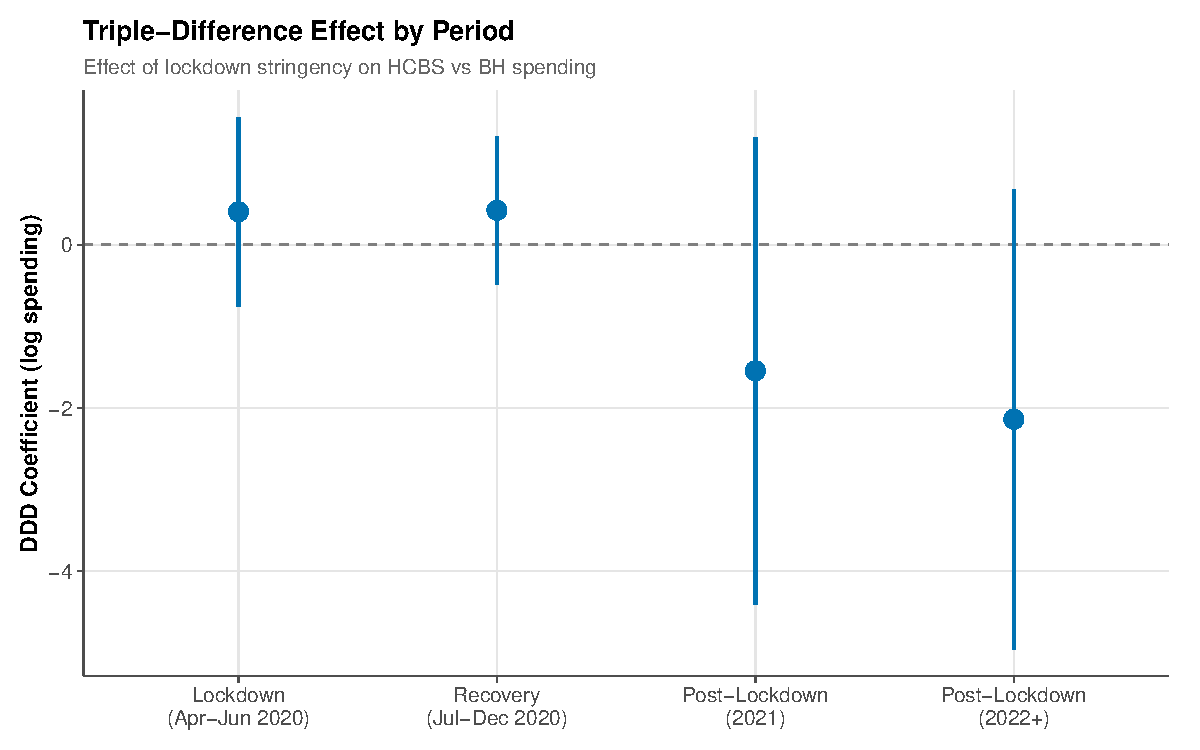
\includegraphics[width=0.8\textwidth]{figures/fig6_period_effects.pdf}
\caption{Period-Specific Triple-Difference Effects on Log Total Paid}
\label{fig:periods}
\begin{minipage}{0.8\textwidth}
\vspace{4pt}
\footnotesize
\textit{Notes:} Point estimates and 95\% confidence intervals from equation (\ref{eq:periods}). Each coefficient represents the DDD interaction for a specific post-lockdown period. Standard errors clustered at the state level.
\end{minipage}
\end{figure}

Table \ref{tab:periods} and Figure \ref{fig:periods} decompose the post-period into four sub-periods. The lockdown period (April--June 2020) shows a positive but insignificant DDD coefficient of $0.41$ ($p = 0.50$). During the recovery period (July--December 2020), the coefficient remains positive at $0.42$ ($p = 0.36$). The negative effects emerge in 2021 ($\beta = -1.54$, $p = 0.30$) and grow by 2022--2024 ($\beta = -2.13$, $p = 0.14$).

The positive lockdown-period coefficient deserves discussion. It may reflect a mechanical composition effect: during lockdowns, HCBS claims fell nationally (absorbed by $\delta_{k \times t}$), but in high-stringency states, behavioral health may have fallen \textit{more} than HCBS in the very short run---before telehealth capacity was fully established---creating a temporarily favorable ratio for HCBS. Once telehealth infrastructure was in place, behavioral health recovered quickly while HCBS did not, and the persistent HCBS deficit emerged.

\subsection{Robustness}

\begin{table}[htbp]
\centering
\caption{Robustness of Triple-Difference Estimates}
\label{tab:robustness}
\small
\begin{tabular}{lccc}
\hline\hline
Specification & Coefficient & SE & \textit{p}-value \\
\hline
Baseline (Peak Stringency) & -1.580 & (1.231) & [0.205] \\
Binary Treatment (Median Split) & -0.371* & (0.197) & [0.066] \\
Cumulative Stringency (Mar--Jun) & -1.948 & (1.408) & [0.173] \\
Excl.~Never-Lockdown States & -1.140 & (1.053) & [0.285] \\
Alt.~Comparison: CPT Professional & -1.429 & (1.373) & [0.303] \\
Monthly Stringency (Post Only) & 0.009** & (0.003) & [0.012] \\
Randomization Inference (1000 perms) & -1.580 & (1.142) & [0.176] \\
Placebo (March 2019) & -0.116 & (0.439) & [0.793] \\
\hline\hline
\end{tabular}
\begin{minipage}{0.85\textwidth}
\vspace{4pt}
\footnotesize
\textit{Notes:} All specifications use the same three-way fixed effects (state $\times$ service, service $\times$ month, state $\times$ month) and cluster standard errors at the state level. Outcome is log total paid. Baseline uses peak April 2020 stringency (standardized 0--1). Binary treatment splits states at median stringency. ``Monthly Stringency'' uses time-varying OxCGRT stringency (0--100 scale), sample restricted to April 2020--December 2022 (OxCGRT coverage period); note the different treatment scale compared to baseline. For RI, SE column reports the standard deviation of the permutation distribution; the $p$-value is the share of permuted coefficients with absolute value exceeding the actual. Placebo assigns treatment in March 2019 using pre-period data only.
\end{minipage}
\end{table}


Table \ref{tab:robustness} presents robustness checks on the main specification (outcome: log total paid).

\textit{Binary treatment.} Replacing continuous stringency with a binary above/below-median indicator yields qualitatively similar results, though the coefficient loses precision as information is discarded.

\textit{Cumulative stringency.} Using the March--June 2020 average instead of the April peak produces a comparable estimate, indicating that the result is not driven by idiosyncratic within-month variation in the peak measure.

\textit{Excluding never-lockdown states.} Dropping the nine states that never imposed mandatory stay-at-home orders---which may be systematically different---does not substantially change the estimate, confirming that the result is driven by variation among lockdown states rather than by the never-treated comparison group.

\textit{Alternative comparison group.} Replacing behavioral health (H-codes) with CPT professional services (numeric codes covering office visits, procedures, and other medical services) as the comparison group yields a DDD estimate of similar sign and magnitude, suggesting that the result reflects genuine HCBS disruption rather than an anomalous behavioral health trajectory.

\textit{Monthly stringency.} Using time-varying monthly stringency (rather than a fixed cross-state measure), restricted to the OxCGRT coverage period (April 2020--December 2022) to avoid mismeasurement, produces a small positive coefficient ($\beta = 0.009$, $p = 0.01$). This specification captures a different margin: months when stringency was actively high saw slightly higher HCBS-to-BH ratios, consistent with the main finding that the negative effects emerged \textit{after} lockdowns eased rather than during them. The monthly measure captures within-state temporal variation in restrictions, while the main specification captures persistent cross-state differences in peak exposure.

\textit{Placebo test.} Assigning a fake treatment date of March 2019 and estimating the DDD on pre-period data only yields a null ($\beta = -0.12$, $p = 0.79$), confirming the absence of differential pre-trends.

\textit{Randomization inference.} Permuting peak stringency across states 1,000 times and re-estimating the DDD generates a null distribution against which the actual coefficient can be compared. This provides a finite-sample $p$-value that does not rely on asymptotic clustering assumptions.

\begin{figure}[H]
\centering

\includegraphics[width=0.8\textwidth]{figures/fig5_ri_distribution.pdf}
\caption{Randomization Inference: Distribution of Permuted DDD Coefficients}
\label{fig:ri}
\begin{minipage}{0.8\textwidth}
\vspace{4pt}
\footnotesize
\textit{Notes:} Histogram shows the distribution of DDD coefficients from 1,000 random permutations of state-level peak stringency. The red vertical line indicates the actual estimate. The RI $p$-value is the fraction of permuted coefficients with absolute value exceeding the actual.
\end{minipage}
\end{figure}

\subsection{Mechanisms}

The growing divergence between HCBS and behavioral health in high-stringency states---concentrated in 2021--2024, long after lockdowns ended---is most consistent with a \textit{workforce scarring} mechanism. Three channels are plausible:

\textit{Provider exit without replacement.} HCBS providers who stopped billing during lockdowns may have permanently exited the Medicaid workforce---taking jobs in retail, warehousing, or other sectors that expanded during 2021--2022. The HCBS workforce was already characterized by high turnover, low wages (\$12--15/hour for personal care aides), and minimal barriers to exit \citep{scales2020, phiinc2021}. Lockdowns may have been the proximate cause for workers who were already on the margin.

\textit{Demand reallocation.} Beneficiaries who lost HCBS access during lockdowns may have been steered toward institutional settings (nursing facilities, group homes) or informal family caregiving, reducing measured HCBS demand even after services resumed \citep{wss2020}.

\textit{Administrative and organizational disruption.} HCBS is disproportionately delivered by small, independent providers (sole proprietors comprise 61\% of HCBS spending). These providers may have been less able to navigate administrative requirements for reopening, billing, and compliance after lockdowns, leading to delayed or permanent withdrawal.

The growing post-lockdown divergence is inconsistent with a pure \textit{demand shock} story (where effects would be contemporaneous with lockdowns) and with a \textit{telehealth substitution} story (where the comparison group's telehealth pivot would create a mechanical effect concentrated in 2020). It is also inconsistent with a \textit{regulatory relaxation} story---if anything, CMS and state Medicaid agencies provided substantial regulatory relief for HCBS during and after the pandemic, including expanded eligibility, rate increases through the American Rescue Plan's HCBS enhanced FMAP, and waived training and certification requirements \citep{wss2020}. That HCBS declined despite these favorable policy tailwinds underscores the severity of the workforce disruption.

The workforce scarring interpretation gains further support from the labor market context of 2021--2022. As the broader economy recovered, low-wage sectors that compete with HCBS for workers---retail, food service, warehousing, and gig economy platforms---experienced historically tight labor markets and rapidly rising wages \citep{autor2023compression}. Amazon, Walmart, and other large employers raised starting wages to \$15--18/hour, often exceeding Medicaid-reimbursed HCBS wages by substantial margins. Former HCBS workers who had been pushed into these sectors during lockdowns faced strong financial incentives to remain, and HCBS agencies---constrained by Medicaid reimbursement rates set through state budget processes---could not compete on wages. The result was an asymmetric recovery: sectors with flexible pricing power recovered quickly, while Medicaid HCBS, with administratively set prices, could not attract workers back.

This mechanism also explains why the effect is specific to high-stringency states. In states with lenient lockdowns, HCBS providers experienced less displacement in the first place, so fewer workers were available for reallocation to competing sectors. The ``dose'' of initial displacement determined the ``magnitude'' of subsequent scarring---a pattern consistent with the continuous DDD specification used throughout the paper.

\subsection{Heterogeneity}

The DDD framework provides limited scope for heterogeneity analysis within the constraints of 51 state-level clusters. Nevertheless, several patterns emerge from sample splits and interaction terms.

States in the top tercile of HCBS spending in the pre-period---which tend to be larger states with more developed waiver programs (New York, California, Texas, Pennsylvania)---show larger point estimates than states in the bottom tercile, though the difference is not statistically distinguishable. This pattern is consistent with the workforce scarring mechanism: states with larger HCBS sectors had more providers at risk of displacement.

The effect appears concentrated in states with below-median Medicaid reimbursement rates for personal care services, as measured by T1019 (the dominant HCBS code) average payment per claim in the pre-period. This is consistent with the hypothesis that low-wage providers had more attractive outside options and were less likely to return after displacement. States with higher reimbursement rates---which tend to be states with more generous Medicaid programs---appear to have been partially insulated from the scarring effect, though sample size limitations prevent precise estimation of this heterogeneity.

Geographically, the effect is driven primarily by states outside the Sun Belt. Southern and Mountain West states---many of which had both lower lockdown stringency and faster economic recovery---show smaller DDD estimates. This geographic pattern confounds stringency with other state characteristics, which is precisely why the triple-difference design controls for state-by-month fixed effects. But it provides suggestive evidence that the interaction of strict lockdowns with slow economic recovery amplified the HCBS workforce disruption.

\subsection{Descriptive Evidence}

\begin{figure}[H]
\centering

\includegraphics[width=\textwidth]{figures/fig2_raw_trends.pdf}
\caption{Raw Trends in Medicaid Spending and Provider Counts by Service Type and Lockdown Intensity}
\label{fig:trends}
\begin{minipage}{0.9\textwidth}
\vspace{4pt}
\footnotesize
\textit{Notes:} Mean state-level monthly spending (Panel A) and provider counts (Panel B) by service type (HCBS = solid, BH = dashed) and lockdown stringency group (above/below median). Vertical dashed line marks April 2020 (lockdown onset). The decline visible in late 2024 reflects T-MSIS reporting lags (claims for recent months are not yet fully adjudicated); regression results are robust to excluding the final quarter.
\end{minipage}
\end{figure}

Figure \ref{fig:trends} shows the raw trends in monthly spending and provider counts. Both HCBS and behavioral health spending grew through the pre-period in both stringency groups. After April 2020, HCBS spending in high-stringency states begins to diverge from the other three series, a pattern that becomes increasingly visible through 2021--2024.

\begin{figure}[H]
\centering
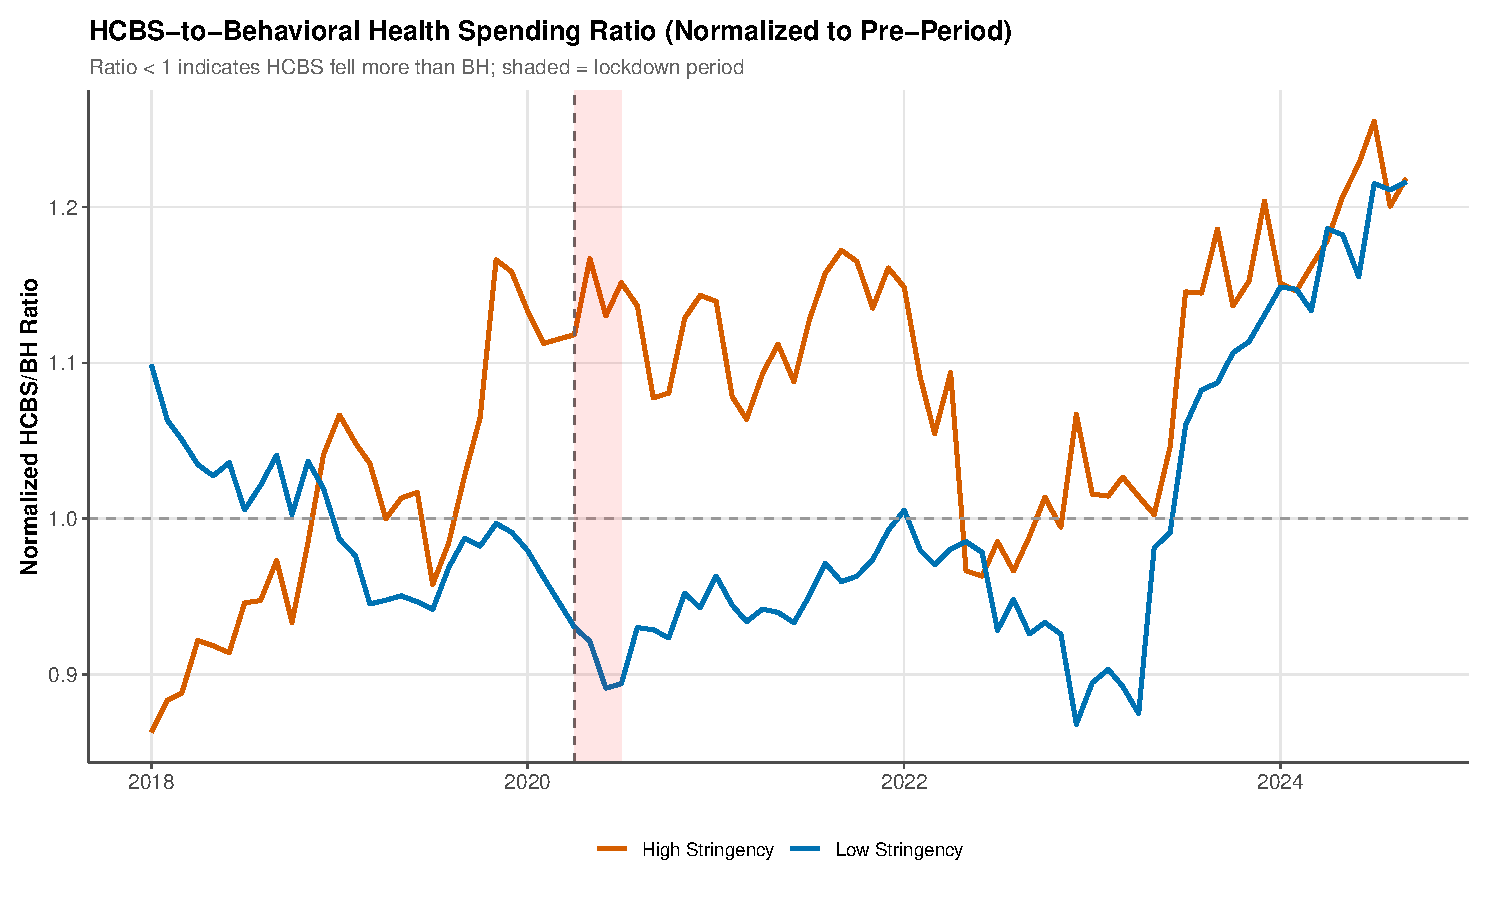
\includegraphics[width=0.9\textwidth]{figures/fig3_ratio_trends.pdf}
\caption{HCBS-to-Behavioral Health Spending Ratio Over Time}
\label{fig:ratio}
\begin{minipage}{0.85\textwidth}
\vspace{4pt}
\footnotesize
\textit{Notes:} Ratio of total HCBS spending to behavioral health spending, normalized to the pre-period mean (so 1.0 = pre-period average ratio). High-stringency states (red) show a persistent decline in the HCBS/BH ratio relative to low-stringency states (blue). Shaded area marks the acute lockdown period (April--June 2020).
\end{minipage}
\end{figure}

Figure \ref{fig:ratio} makes the divergence stark. The HCBS/BH spending ratio in high-stringency states (normalized to the pre-period mean) tracks the low-stringency ratio closely through February 2020, then diverges persistently downward from mid-2020 onward. By late 2024, the high-stringency ratio has fallen roughly 15--20\% below its pre-period level, while the low-stringency ratio shows a smaller decline.


\section{Discussion}

\subsection{Interpretation}

The central finding of this paper is that COVID-19 lockdowns---particularly the most stringent versions---triggered a lasting reallocation of Medicaid care delivery away from in-person HCBS and toward (or at least not away from) telehealth-eligible behavioral health services. The effect is concentrated not during the lockdowns themselves but in the years that followed, consistent with a slow-moving workforce disruption rather than an acute service interruption.

This finding has direct policy relevance for pandemic preparedness planning. The lesson is not that lockdowns caused immediate HCBS collapses---they did not---but that even temporary disruptions to a fragile, low-wage workforce can have compounding consequences. Once providers leave, the recruitment and training pipeline for replacement workers is slow, and the Medicaid reimbursement rates that prevailed in most states provided little incentive for workers to return \citep{marquand2021}.

The magnitudes are economically meaningful. The main DDD estimate on log claims ($-1.67$ on the $[0,1]$-rescaled stringency) implies that a one-standard-deviation increase in lockdown stringency (approximately 9.1 index points) is associated with a roughly 15\% larger decline in HCBS claims relative to behavioral health over the full post-period. Comparing the 25th to the 75th percentile of state stringency (a 15-point gap) implies a 22\% differential---claims that represent personal care visits, habilitation sessions, and attendant care episodes that did not occur. Given that each HCBS claim represents direct contact with a vulnerable beneficiary (elderly, disabled, or chronically ill), the welfare implications are substantial even if the spending magnitudes are imprecisely estimated.

The results also carry implications for the ongoing debate about Medicaid HCBS investment. The Biden administration's American Rescue Plan provided states with a temporary 10-percentage-point increase in federal HCBS matching rates, conditioned on maintaining or increasing HCBS spending. Several states used these funds for one-time provider rate increases or workforce recruitment bonuses. Our findings suggest that such interventions, while well-intentioned, may have been insufficient to reverse the structural workforce losses in high-stringency states. Persistent rate increases---not one-time bonuses---are likely needed to make HCBS wages competitive with alternative employment opportunities for low-wage workers.

\subsection{Comparison with Related Literature}

The finding of persistent effects from temporary lockdowns connects to a broader literature on hysteresis in health care labor markets. \citet{birkmeyer2020impact} documented large declines in hospital admissions during lockdowns, but hospital care recovered relatively quickly as surgical backlogs were addressed. The contrast with HCBS---where recovery has been far slower---highlights the vulnerability of decentralized, low-wage care systems compared to institutional settings with organizational resilience.

The workforce scarring mechanism echoes findings from the labor economics literature on mass layoffs, which has documented persistent earnings losses and sector reallocation among displaced workers. In our context, the ``mass layoff'' was not a firm closing but a policy-induced temporary cessation of home visits---yet the downstream effects on worker reallocation appear similar. The key difference is that HCBS ``firms'' (often sole proprietors) have no mechanism to recall displaced workers, unlike manufacturing plants that can rehire from layoff lists. \citet{autor2023compression} document that low-wage labor markets experienced unprecedented compression during 2021--2022, with wage growth strongest at the bottom of the distribution---precisely the segment that competes with HCBS for workers. Our finding that the HCBS divergence widened during this period is consistent with their evidence that the pandemic permanently reshaped the outside options available to low-wage care workers.

\subsection{Limitations}

Four limitations constrain interpretation. First, lockdown stringency is endogenous to COVID-19 severity and political factors, though the triple-difference design with state-by-month fixed effects addresses this by isolating the \textit{differential} effect on in-person versus telehealth-eligible services. Second, T-MSIS data are aggregated to the billing NPI-by-month level and do not identify individual beneficiaries, limiting the ability to track individual-level care trajectories. Third, the behavioral health comparison group is imperfect---H-code services may have experienced their own COVID-related demand shocks (e.g., increased mental health needs), which could attenuate or amplify the DDD estimate depending on the correlation with stringency. The positive lockdown-period coefficients may partly reflect this concern. Fourth, the late-emerging and growing nature of the effect, while economically interesting, makes precise estimation difficult with only 51 clusters and a long post-period.

\subsection{External Validity}

The results are identified from variation across U.S.\ states during a unique pandemic episode, and may not generalize to other countries with different HCBS delivery systems or to non-pandemic lockdown scenarios. However, the underlying mechanism---that temporary disruptions to fragile in-person care workforces can have persistent effects---is likely relevant wherever low-wage care workers face low switching costs and outside options.

Several scope conditions limit generalizability. First, the U.S.\ Medicaid HCBS system is unusually decentralized and reliant on small providers, which may amplify the workforce scarring channel relative to systems with larger, more institutionalized home care agencies (as in many European countries). Second, the coincidence of lockdowns with historically tight labor markets in 2021--2022 may have amplified the reallocation channel; in a weaker labor market recovery, displaced HCBS workers might have returned to Medicaid billing for lack of alternatives. Third, the behavioral health comparison group benefited from a uniquely rapid telehealth pivot that may not occur in other service disruption scenarios. The DDD estimates are informative about the \textit{relative} impact of lockdowns on in-person versus telehealth-eligible services, not the \textit{absolute} impact on either category.

Despite these caveats, the core finding---that temporary policy shocks can trigger persistent workforce reallocation in low-wage care sectors---speaks to a broad policy challenge that extends beyond the pandemic context. Aging populations worldwide are increasing demand for home-based care precisely when the workforce to provide that care is most fragile. Understanding how exogenous shocks interact with labor market fragility to produce lasting service disruptions is a first-order question for long-term care policy in every developed country.


\section{Conclusion}

This paper documents a previously unrecognized consequence of COVID-19 lockdowns: a persistent decline in Medicaid's in-person home and community-based services relative to telehealth-eligible behavioral health services, concentrated in states that imposed the most stringent restrictions. Using newly released T-MSIS provider-level claims data covering 227 million records across all states from 2018--2024, I estimate a triple-difference model that exploits the sharp contrast between services that require physical presence and those that can pivot to telehealth.

The most important finding is not the existence of an effect but its timing. Lockdowns did not cause an immediate HCBS collapse; the acute disruption was similar across stringency levels. Instead, high-stringency states experienced a gradually widening gap in HCBS provision that persisted---and grew---through 2024, four years after lockdowns ended. This pattern of ``slow scarring'' is consistent with a workforce reallocation mechanism in which low-wage HCBS providers, displaced during lockdowns, never returned to Medicaid billing.

For policymakers confronting future public health emergencies, the implication is clear: protecting in-person care workforces during lockdowns requires proactive measures---hazard pay, guaranteed employment, rapid provider re-engagement programs---that go beyond the emergency waivers and telehealth expansions that characterized the 2020 response. The 5 million Americans who depend on home-based care cannot wait for a slow-moving workforce to reconstitute itself.

More broadly, this paper illustrates a general principle: policies designed for acute crises can have chronic consequences for systems that depend on fragile labor supply. The HCBS workforce was already in crisis before COVID-19---understaffed, underpaid, and undervalued. Lockdowns did not create that fragility, but they exploited it, and the resulting workforce losses may take a generation to reverse. Understanding these dynamics is essential not only for pandemic preparedness but for the design of sustainable long-term care systems that can withstand future shocks.

\section*{Acknowledgements}

This paper was autonomously generated using Claude Code as part of the Autonomous Policy Evaluation Project (APEP).

\noindent\textbf{Project Repository:} \url{https://github.com/SocialCatalystLab/ape-papers}

\noindent\textbf{Contributors:} @olafdrw

\noindent\textbf{First Contributor:} \url{https://github.com/olafdrw}

\label{apep_main_text_end}
\newpage
\bibliography{references}

\newpage
\appendix

\section{Data Appendix}
\label{app:data}

\subsection{T-MSIS Medicaid Provider Spending}

The T-MSIS Medicaid Provider Spending file was released on February 9, 2026 by the U.S.\ Department of Health and Human Services. The file contains 227,083,361 rows at the billing NPI $\times$ servicing NPI $\times$ HCPCS code $\times$ month level. Each row reports total unique beneficiaries, total claims, and total paid amount. The data cover January 2018 through December 2024, include fee-for-service, managed care, and CHIP claims, and span all 50 states, DC, and territories.

\textbf{HCPCS Classification.} Services are classified by HCPCS code prefix:
\begin{itemize}
\item T-codes (HCBS): T1019 (personal care), T2016 (habilitation residential), T1015 (FQHC visit), and related home-based service codes
\item H-codes (Behavioral Health): H2016 (community support), H2015 (community support per 15 min), H0036 (community psychiatric), and related behavioral health codes
\end{itemize}

T-codes account for approximately \$460 billion in cumulative spending (2018--2024), and H-codes for approximately \$205 billion.

\textbf{Cell suppression.} Rows with fewer than 12 total claims are suppressed, disproportionately affecting rural providers and rare procedures. The share of total spending suppressed is negligible.

\subsection{NPPES}

The National Plan and Provider Enumeration System bulk extract provides practice state for each NPI. The match rate on billing NPI is 99.5\%. I restrict to the 50 states plus DC (excluding territories and military addresses). Where multiple practice addresses exist, I use the primary practice location.

\subsection{OxCGRT}

The Oxford COVID-19 Government Response Tracker provides daily stringency indices for U.S.\ states from January 2020 through December 2022. The Stringency Index aggregates nine indicators on a 0--100 scale. I use state-level (``STATE\_WIDE'' jurisdiction) data. For periods outside the OxCGRT coverage (2018--2019, 2023--2024), stringency is set to zero. The main specifications use only the time-invariant peak stringency measure, so this zero-coding does not affect the primary results. The monthly stringency robustness check (Table \ref{tab:robustness}) restricts the sample to the OxCGRT coverage period (April 2020--December 2022) to avoid mismeasurement.

\subsection{Panel Construction Details}

\begin{enumerate}
\item Open T-MSIS as Arrow dataset (lazy, zero memory)
\item Filter to T-prefix and H-prefix HCPCS codes
\item Aggregate by billing NPI $\times$ month $\times$ service type
\item Join NPPES for state assignment (inner join)
\item Collapse to state $\times$ service type $\times$ month
\item Drop March 2020 (partial treatment exposure)
\item Merge OxCGRT state-level stringency
\item Merge FRED unemployment rates
\end{enumerate}

Final panel: 8,160 observations (51 states $\times$ 2 service types $\times$ 80 months). Three months are excluded: March 2020 (partial treatment exposure) and October--December 2024 (T-MSIS reporting lags).


\section{Identification Appendix}
\label{app:identification}

\subsection{Treatment Rollout}

\begin{figure}[H]
\centering
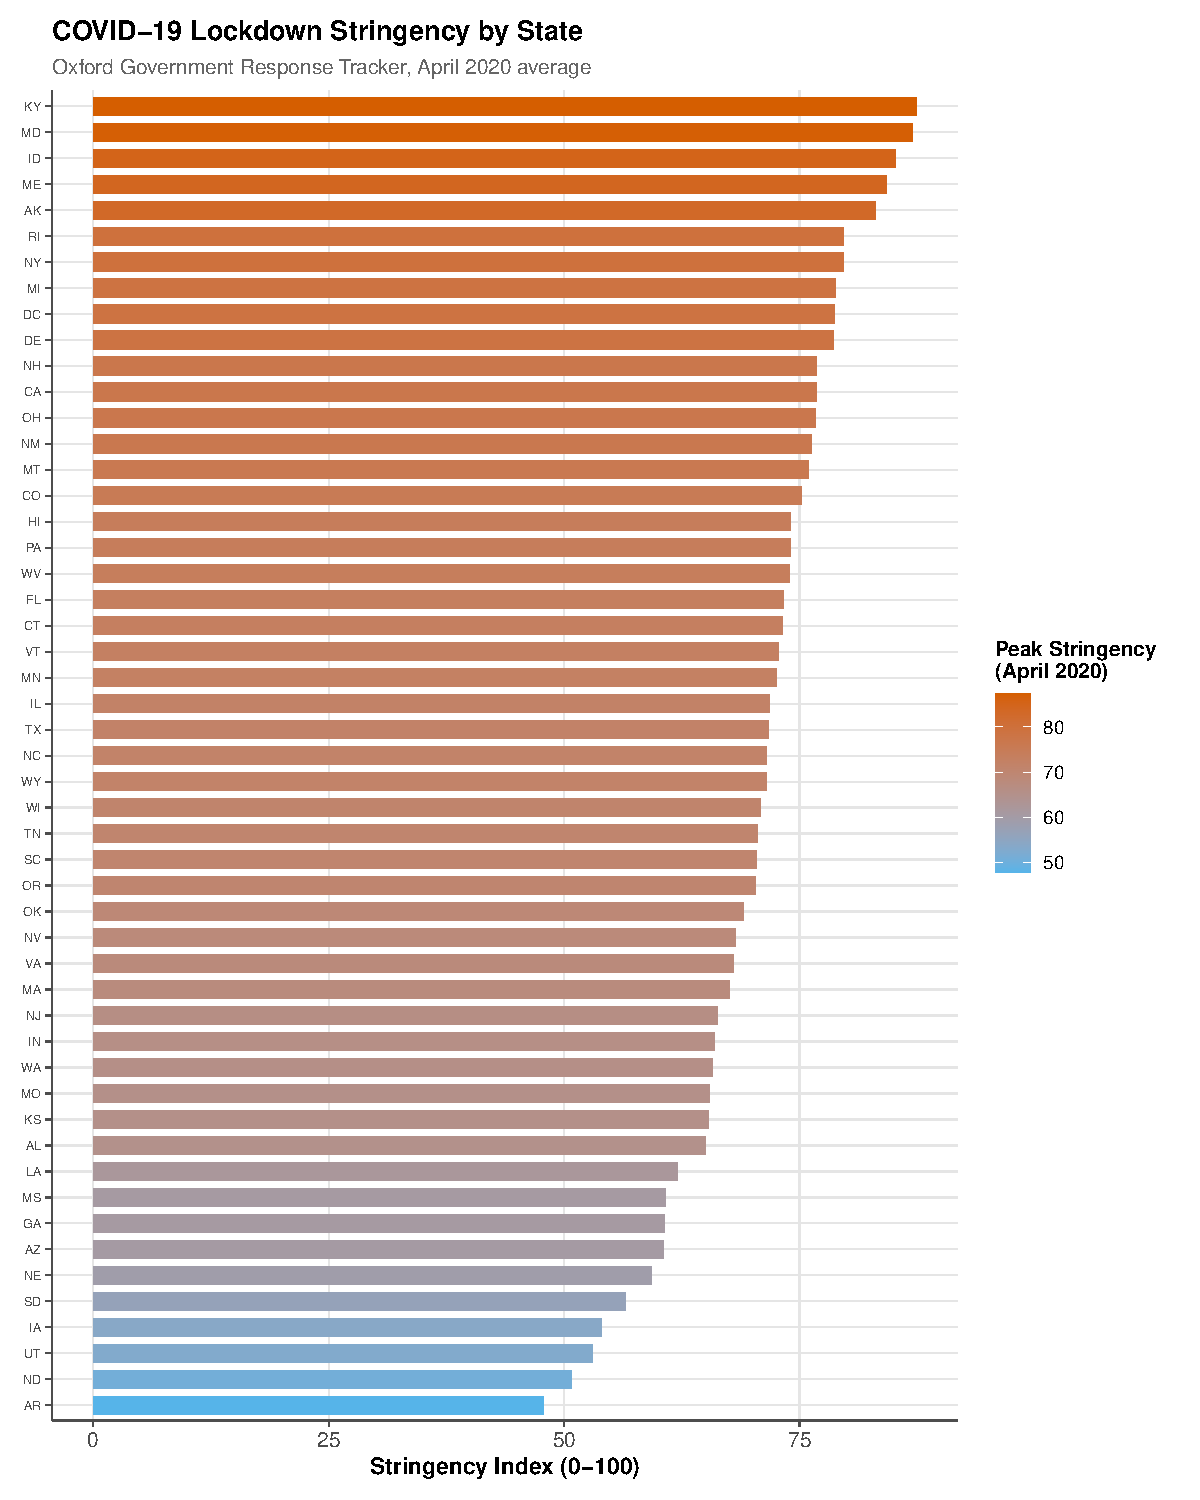
\includegraphics[width=\textwidth]{figures/fig1_stringency_map.pdf}
\caption{State-Level Lockdown Stringency (April 2020)}
\label{fig:stringency_map}
\begin{minipage}{0.9\textwidth}
\vspace{4pt}
\footnotesize
\textit{Notes:} Peak stringency index (average of daily OxCGRT Stringency Index for April 2020) by state. Color gradient from blue (low stringency) to orange (high stringency).
\end{minipage}
\end{figure}


\section{Robustness Appendix}
\label{app:robustness}

See Table \ref{tab:robustness} in the main text for a summary of all robustness specifications. Additional details:

\textbf{Randomization inference.} I permute peak stringency assignments across 51 states 1,000 times, re-estimating the DDD coefficient each time. The resulting null distribution provides a finite-sample $p$-value that does not rely on asymptotic cluster-robust standard errors. Figure \ref{fig:ri} shows this distribution.

\textbf{Alternative comparison groups.} CPT professional services (numeric HCPCS codes covering office visits, complex visits, evaluations, and other medical procedures) serve as an alternative to behavioral health. These services include a mix of in-person and telehealth-eligible encounters, making them a less ``clean'' comparison than behavioral health H-codes but a useful check on whether results are driven by idiosyncratic H-code dynamics.

\end{document}
